% This file was converted to LaTeX by Writer2LaTeX ver. 1.0.2
% see http://writer2latex.sourceforge.net for more info
\documentclass[a4paper]{article}
\usepackage[utf8]{inputenc}
\usepackage[T1]{fontenc}
\usepackage[english,portuges]{babel}
\usepackage{amsmath}
\usepackage{amssymb,amsfonts,textcomp}
\usepackage{color}
\usepackage{array}
\usepackage{hhline}
\usepackage{hyperref}
\hypersetup{pdftex, colorlinks=true, linkcolor=blue, citecolor=blue, filecolor=blue, urlcolor=blue, pdftitle=, pdfauthor=Antonio Carlos Falcão Petri, pdfsubject=, pdfkeywords=}
\usepackage[pdftex]{graphicx}
% List styles
\newcounter{saveenum}
\newcommand\liststyleWWNumv{%
\renewcommand\labelitemi{[F0B7?]}
\renewcommand\labelitemii{o}
\renewcommand\labelitemiii{[F0A7?]}
\renewcommand\labelitemiv{[F0B7?]}
}
\newcommand\liststyleWWNumvii{%
\renewcommand\labelitemi{[F0B7?]}
\renewcommand\labelitemii{o}
\renewcommand\labelitemiii{[F0A7?]}
\renewcommand\labelitemiv{[F0B7?]}
}
\newcommand\liststyleWWNumiii{%
\renewcommand\theenumi{\arabic{enumi}}
\renewcommand\theenumii{\alph{enumii}}
\renewcommand\theenumiii{\roman{enumiii}}
\renewcommand\theenumiv{\arabic{enumiv}}
\renewcommand\labelenumi{\theenumi.}
\renewcommand\labelenumii{\theenumii.}
\renewcommand\labelenumiii{\theenumiii.}
\renewcommand\labelenumiv{\theenumiv.}
}
\newcommand\liststyleWWNumiv{%
\renewcommand\labelitemi{[F0B7?]}
\renewcommand\labelitemii{o}
\renewcommand\labelitemiii{[F0A7?]}
\renewcommand\labelitemiv{[F0B7?]}
}
\newcommand\liststyleWWNumvi{%
\renewcommand\labelitemi{[F0B7?]}
\renewcommand\labelitemii{o}
\renewcommand\labelitemiii{[F0A7?]}
\renewcommand\labelitemiv{[F0B7?]}
}
% Page layout (geometry)
\setlength\voffset{-1in}
\setlength\hoffset{-1in}
\setlength\topmargin{1.1811in}
\setlength\oddsidemargin{1.1811in}
\setlength\textheight{9.7244in}
\setlength\textwidth{6.2995996in}
\setlength\footskip{0.0cm}
\setlength\headheight{0cm}
\setlength\headsep{0cm}
% Footnote rule
\setlength{\skip\footins}{0.0469in}
\renewcommand\footnoterule{\vspace*{-0.0071in}\setlength\leftskip{0pt}\setlength\rightskip{0pt plus 1fil}\noindent\textcolor{black}{\rule{0.0\columnwidth}{0.0071in}}\vspace*{0.0398in}}
% Pages styles
\makeatletter
\newcommand\ps@Standard{
  \renewcommand\@oddhead{}
  \renewcommand\@evenhead{}
  \renewcommand\@oddfoot{}
  \renewcommand\@evenfoot{}
  \renewcommand\thepage{\arabic{page}}
}
\makeatother
\pagestyle{Standard}
\newcounter{Imagem2}
\renewcommand\theImagem2{\arabic{Imagem2}}
\newcounter{Imagem1}
\renewcommand\theImagem1{\arabic{Imagem1}}
\title{}
\author{Antonio Carlos Falcão Petri}
\date{2015-04-23}
\begin{document}
\clearpage\setcounter{page}{1}\pagestyle{Standard}
{\centering 

\includegraphics[width=3.5602in,height=1.7756in]{T1-img1.png} \par}


\bigskip


\bigskip


\bigskip


\bigskip

{\centering
\foreignlanguage{english}{\textbf{The Last: Too Fast}}
\par}


\bigskip


\bigskip


\bigskip


\bigskip

{\raggedleft
\foreignlanguage{english}{\textcolor{black}{Antonio Carlos Falcão Petri
586692}}
\par}

{\raggedleft
\textcolor{black}{José Antônio dos Santos Júnior 586765}
\par}

{\raggedleft
\textcolor{black}{José Vitor de Carvalho Aquino 609170}
\par}

{\raggedleft
\textcolor{black}{Tiago Bonadio Badoco 586722}
\par}


\bigskip


\bigskip


\bigskip


\bigskip


\bigskip


\bigskip


\bigskip


\bigskip


\bigskip


\bigskip


\bigskip


\bigskip


\bigskip

{\centering
\textcolor{black}{São Carlos}
\par}

{\centering
\textcolor{black}{Abril/2015}
\par}

\textbf{Autores:}

Antonio Carlos Falcão Petri
(\href{mailto:falcaopetri@gmail.com}{falcaopetri@gmail.com}) –
Implementação do Jogo

\textcolor{black}{José Antônio dos Santos Júnior}
(\href{mailto:jusantosjr@hotmail.com}{jusantosjr@hotmail.com}) –
Desenvolvimento Gráfico

José Vitor Aquino
(\href{mailto:jvcaquino95@gmail.com}{jvcaquino95@gmail.com}) –
Implementação das Estruturas de Dados

Tiago Bonadio Badoco
(\href{mailto:tiago.badoco@gmail.com}{tiago.badoco@gmail.com}) -
\ Documentação


\bigskip

\textbf{Funcionamento do Jogo:}

O jogo consiste na apresentação de figuras geométricas, uma a uma. Essas
figuras estão armazenadas em uma fila. O usuário deve responder “Sim”
ou “Não” à pergunta “A figura mostrada na tela, é igual à mostrada
anteriormente?”. Assim que ele responder, a figura atual passa a ser a
anterior e uma nova figura é exibida na tela. Se o usuário erra a
resposta, a imagem é adicionada novamente à fila. Além disso, o erro
acarreta uma adição de 5 segundo no tempo de jogo.

Um sistema de dificuldade determina o número de elementos na fila. No
nível fácil são 30 figuras, no médio 50, no difícil 70 e no insano 90.

A pontuação do jogador é baseada em dois diferentes critérios: o tempo
de conclusão e o número de erros. O tempo de conclusão é o fator mais
importante e é ele que define o desempenho. Quanto menor o valor do
tempo de conclusão, melhor o usuário foi na partida. O número de erros
serve como critério de desempate para tempos iguais, sendo que quem
tiver o menor número de erros terá o melhor resultado.


\bigskip

\textbf{Controles:}

Mouse – O mouse controla todas as interações com os menus do jogo,
selecionando as opções desejadas.

Seta Esquerda – A seta para esquerda é utilizada para controlar o jogo
em si, significando que a imagem atual NÃO É igual à anterior.

Seta Direita – Em oposição, a seta para a direita é utilizada dizer que
a imagem atual É igual à anterior.


\bigskip

\textbf{\ \ Ferramentas:}

\liststyleWWNumv
\begin{itemize}
\item \textcolor{black}{Codeblocks;}
\item \textcolor{black}{Allegro 5;}
\item \textcolor{black}{Photoshop CS5;}
\item \textcolor{black}{Fruity Loops Producer Edition 11;}
\end{itemize}
\liststyleWWNumvii
\begin{itemize}
\item
\foreignlanguage{english}{\textcolor{black}{STL}}\foreignlanguage{english}{,
C++~Standard Template
Library}\foreignlanguage{english}{\textcolor{black}{. }}
\end{itemize}
\textbf{Telas}:

\liststyleWWNumiii
\begin{enumerate}
\item \textbf{Menu Principal (Imagem 1.1)}
\end{enumerate}
Essa tela apresenta três recursos ao jogador. A seleção da opção
“Iniciar Partida” leva o jogador a tela de seleção de dificuldade. A
opção “Sobre” leva o jogador para uma tela com as informações dos
desenvolvedores. Por fim, o ícone do alto falante permite ao jogador
habilitar ou desabilitar a música de fundo.

{\centering 
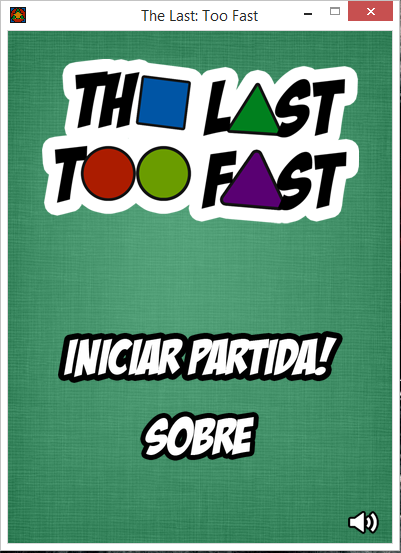
\includegraphics[width=3.148in,height=4.3307in]{T1-img2.png} \par}

{\centering\itshape\color[rgb]{0.26666668,0.32941177,0.41568628}
Imagem 1. \stepcounter{Imagem1}{\theImagem1} - Menu Principal, três
opções estão disponíveis para o usuário
\par}


\bigskip

\liststyleWWNumiii
\setcounter{saveenum}{\value{enumi}}
\begin{enumerate}
\setcounter{enumi}{\value{saveenum}}
\item \textbf{Sobre (Imagem 1.2)}
\end{enumerate}
Essa tela é responsável pela apresentação dos desenvolvedores do jogo.
Nela é apresentada a disciplina que requisitou o projeto bem como o
professor responsável; o nome dos desenvolvedores completos; e a
universidade e ano do desenvolvimento.

{\centering 
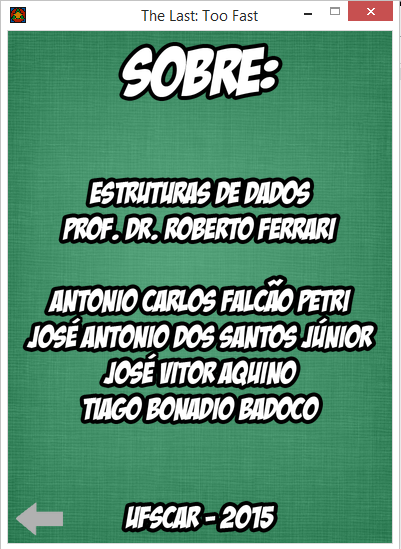
\includegraphics[width=3.1634in,height=4.3307in]{T1-img3.png} \par}

{\centering\itshape\color[rgb]{0.26666668,0.32941177,0.41568628}
Imagem 1. \stepcounter{Imagem1}{\theImagem1} - Tela
{\textquotedbl}Sobre{\textquotedbl} apresenta informações dos
desenvolvedores
\par}


\bigskip

\liststyleWWNumiii
\setcounter{saveenum}{\value{enumi}}
\begin{enumerate}
\setcounter{enumi}{\value{saveenum}}
\item \textbf{Selecionar Dificuldade (Imagem 1.3)}
\end{enumerate}
Nessa tela são apresentados seis recursos ao jogador. Há a persistência
do botão de alto falante, presente no Menu Principal; uma seta que
permite ao jogador retornar ao Menu Principal; e quatro opções de
dificuldade, que alteram as definições do jogo buscando proporcionar
uma experiência mais desafiadora ao usuário:

\liststyleWWNumiv
\begin{itemize}
\item Fácil: \ \  São 30 figuras geométricas na fila.
\item Médio: São 50 figuras geométricas na fila.
\item Difícil: São 70 figuras geométricas na fila.
\item Insano: São 90 figuras geométricas na fila.
\end{itemize}
A seleção de qualquer uma das dificuldades leva o jogador para a tela
Jogo.


\bigskip


\bigskip

{\centering 
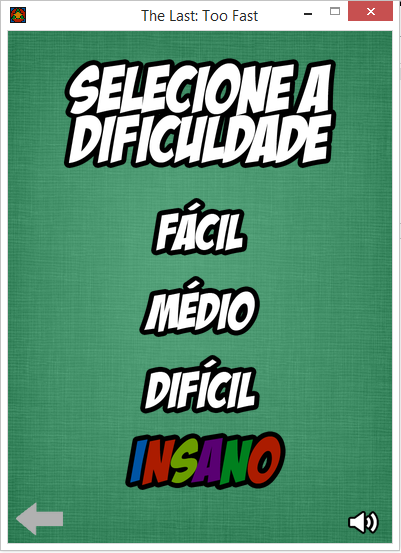
\includegraphics[width=3.1402in,height=4.3307in]{T1-img4.png} \par}

{\centering\itshape\color[rgb]{0.26666668,0.32941177,0.41568628}
Imagem 1. \stepcounter{Imagem1}{\theImagem1} - A tela
{\textquotedbl}Selecionar Dificuldade{\textquotedbl} permite ao usuário
selecionar o nível mais conveniente para suas habilidades
\par}


\bigskip

\liststyleWWNumiii
\begin{enumerate}
\item \textbf{Jogo (Imagens 1.4 e 1.5)}
\end{enumerate}
A tela Jogo inicia com uma figura geométrica na tela, nada mais. Após
alguns instantes a figura geométrica se altera (ou não) e uma mensagem
surge na tela perguntando se a imagem é igual a anterior. Na parte
inferior uma mensagem orienta o jogador sobre como controlar o jogo. A
seta para esquerda diz que a imagem não é igual a anterior, a seta para
direita diz que a imagem é igual a anterior. A tela Jogo com essas
informações pode ser vista na Imagem 1.4:


\bigskip

{\centering 
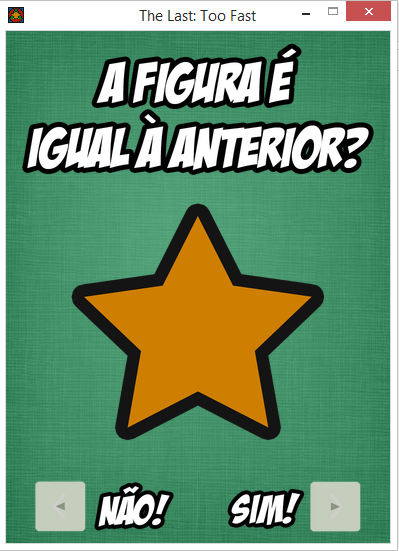
\includegraphics[width=3.1362in,height=4.3307in]{T1-img5.png} \par}

{\centering\itshape\color[rgb]{0.26666668,0.32941177,0.41568628}
Imagem 1. \stepcounter{Imagem1}{\theImagem1} - Tela
{\textquotedbl}Jogo{\textquotedbl} apresentando instruções do jogo
\par}


\bigskip

Após alguns segundos a mensagem perguntando ao jogador se a figura é
igual à anterior some dando lugar a um timer, que mostra o tempo
decorrido de jogo, e um contador vermelho, que mostra quantas vezes o
usuário já errou. É possível notar a mudança comparando a Imagem 1.4
com a Imagem 1.5.

{\centering 
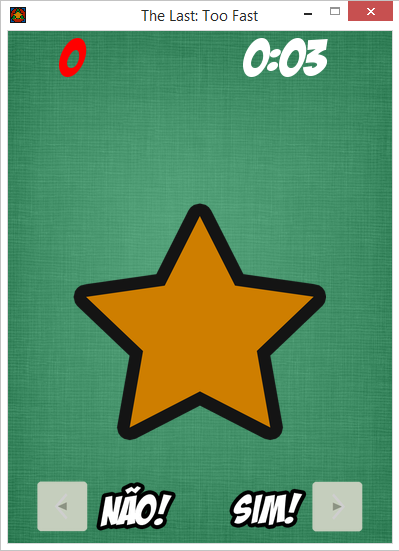
\includegraphics[width=3.1362in,height=4.3307in]{T1-img6.png} \par}

{\centering\itshape\color[rgb]{0.26666668,0.32941177,0.41568628}
Imagem 1. \stepcounter{Imagem1}{\theImagem1} - Tela
{\textquotedbl}Jogo{\textquotedbl} com o timer contabilizando 3
segundos de jogo e o contador de erros em zero
\par}


\bigskip

\liststyleWWNumiii
\setcounter{saveenum}{\value{enumi}}
\begin{enumerate}
\setcounter{enumi}{\value{saveenum}}
\item \textbf{Score (Imagem 1.6)}
\end{enumerate}
A tela Score mostra o resultado final da partida apresentando o tempo
feito pelo jogador e o número de erros. O único recurso nessa tela é
uma seta que leva o jogador para a tela Selecionar Dificuldade, visando
o início de uma nova partida de forma ágil. A tela Score pode ser vista
na Imagem 1.6.

{\centering 
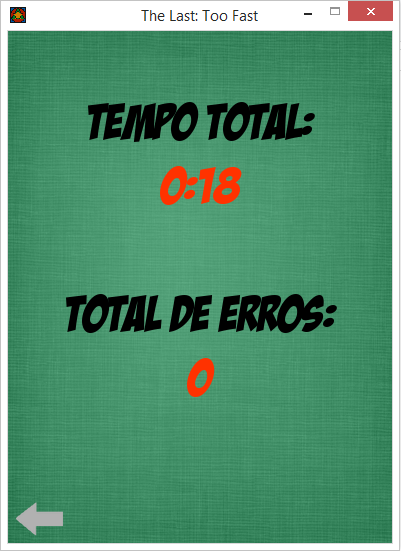
\includegraphics[width=3.1516in,height=4.3307in]{T1-img7.png} \par}

{\centering\itshape\color[rgb]{0.26666668,0.32941177,0.41568628}
Imagem 1. \stepcounter{Imagem1}{\theImagem1} - A Tela
{\textquotedbl}Score{\textquotedbl} apresenta os resultados do usuário
na partida
\par}


\bigskip

\clearpage
\textbf{Diagrama da Arquitetura do Software:}\textbf{ }

O sistema teve sua arquitetura pensada da maneira expressa na Imagem 2.1


  [Warning: Image ignored] % Unhandled or unsupported graphics:
%\includegraphics[width=6.3024in,height=3.3024in]{}
 

{\centering\itshape\color[rgb]{0.26666668,0.32941177,0.41568628}
Imagem 2. \stepcounter{Imagem2}{\theImagem2} - Arquitetura do Sistema
\par}


\bigskip

Os diagramas a seguir buscam ser uma representação visual do sistema,
baseando-se nos Diagramas de Classe, mas sem nenhum rigor. Os itens GUI
e TheLastTooFast, por exemplo, não representam classes do sistema.
Mesmo assim, essa diagramação é apresentada por possuir informações
importantes quanto ao funcionamento do Jogo. O diagrama completo pode
ser encontrado na pasta Documentação, no formato JPEG.

\begin{figure}
\centering
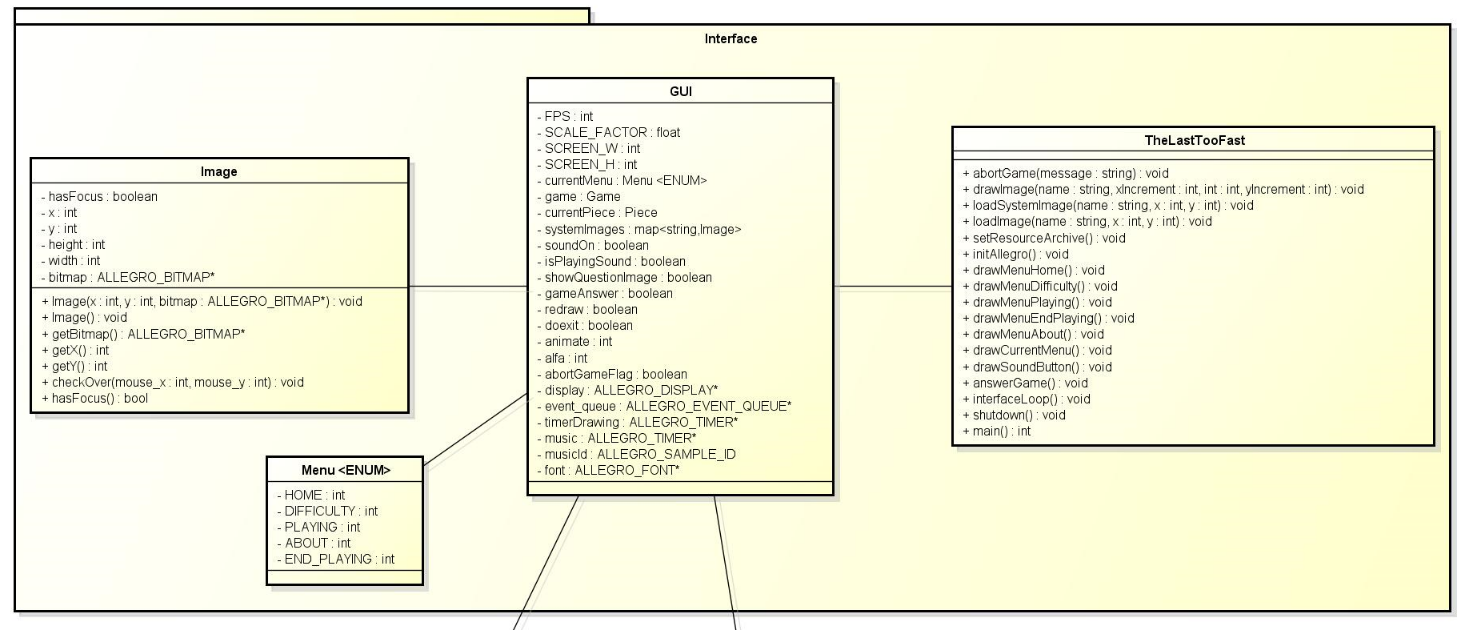
\includegraphics[width=6.6528in,height=2.8634in]{T1-img8.png}
\end{figure}
{\centering\itshape\color[rgb]{0.26666668,0.32941177,0.41568628}
Imagem 2. \stepcounter{Imagem2}{\theImagem2} - Diagrama da Arquitetura
do Software, em relação à sua Interface Gráfica
\par}


\bigskip

Nesse primeiro pacote (Imagem 2.2), tem-se os principais elementos da
Interface Gráfica. O item GUI possui todas as \textit{variáveis} de
controle, sendo incluído pelo item TheLastTooFast, que possui todas as
\textit{funções} de controle do Jogo.

É notável a criação da Classe \textit{Image}, que encapsula um
\textit{ALLEGRO\_BITMAP} (uma imagem carregada pelo Allegro) e
disponibiliza métodos que verificam se a imagem está sobre o foco do
Mouse, permitindo encapsular esse comportamento de forma concisa e
reutilizável ao longo do código da interface. Essa classe possui ainda
informações quanto a sua posição (X, Y) relativas à tela, o que
facilita a realização do \textit{drawing} da imagem.


\bigskip

Na segunda parte do sistema (Imagem 2.3), está encapsulado todo a lógica
do Jogo. Esse pacote é autossuficiente em relação ao pacote Interface,
dependendo apenas dos TADs discutidos a seguir. Aqui, a Figura
Geométrica é abstraída em uma Classe Piece, que possui apenas um
identificador numérico.

\begin{figure}
\centering
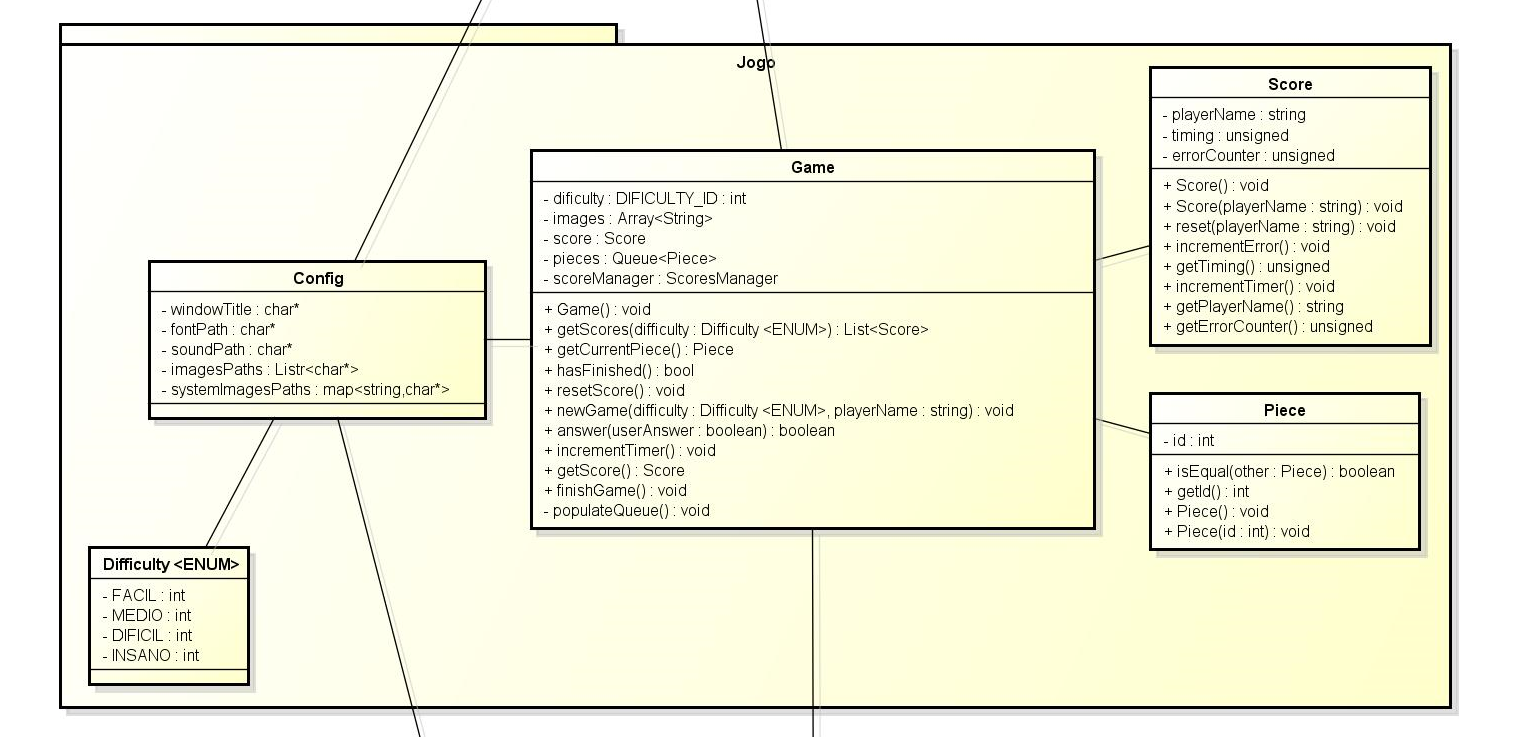
\includegraphics[width=6.2917in,height=3.0626in]{T1-img9.png}
\end{figure}

\bigskip

{\centering\itshape\color[rgb]{0.26666668,0.32941177,0.41568628}
Imagem 2. 3 - Diagrama da Arquitetura do Software, em relação à Lógica
do Jogo
\par}


\bigskip

Por fim, encontram-se as estruturas básicas do jogo, cujas
implementações são a motivação principal do desenvolvimento dessa
aplicação, merecendo uma seção à parte para explicação.



\begin{figure}
\centering
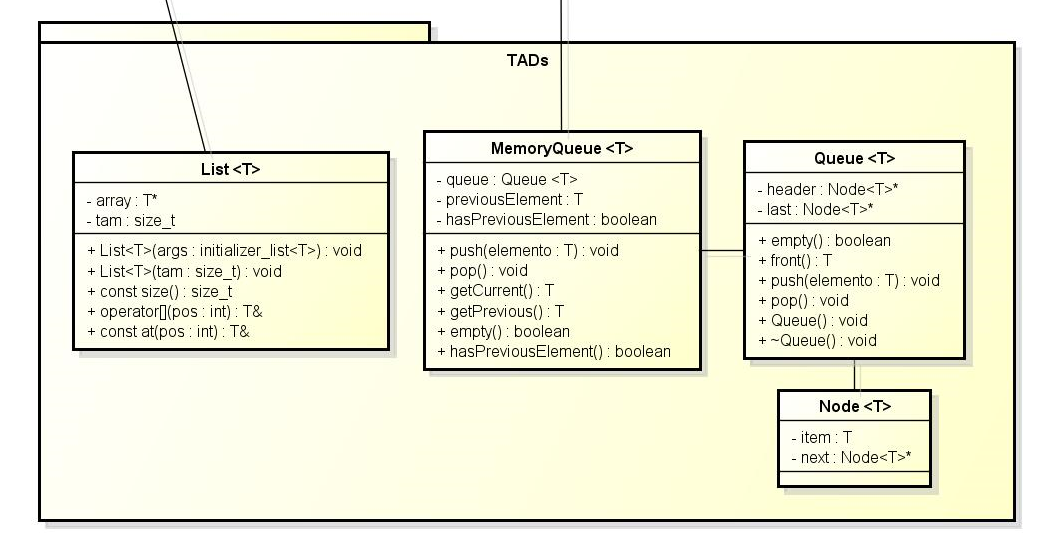
\includegraphics[width=6.302in,height=3.2602in]{T1-img10.png}
\end{figure}
{\centering\itshape\color[rgb]{0.26666668,0.32941177,0.41568628}
Imagem 2. 4 - Diagrama da Arquitetura do Software, em relação às
Estruturas de Dados
\par}


\bigskip

\textbf{TAD’s}

A implementação do jogo utilizada utiliza-se de 3 estruturas de dados
para organizar os principais elementos do jogo. São elas: uma Fila
encapsulada em uma estrutura que foi chamada de MemoryQueue, uma Lista,
e um Map. A estrutura Map não está representada na Imagem 2.4 por não
ter sido implementada pelo grupo. Assim, há apenas um comentário ao
final dessa seção explicando o que é essa estrutura e quais os
benefícios de sua utilização nesse jogo.

É importante ressaltar que as duas estruturas implementadas utilizam o
conceito de Templates, mantendo a camada de abstração entre a estrutura
e os dados que ela armazena. Além disso, teve-se como parâmetro de
implementação as estruturas da STL, referências em C++.

\textbf{Como a Fila é implementada e utilizada?}

A Fila é utilizada para “armazenar as figuras geométricas”. Ela
é\textcolor{black}{ implementada para inserir elementos de forma
dinâmica e encadeada. Assim, surge a Classe Node, que encapsula as
informações referentes ao “item”, e ao endereço de onde está o próximo
item. Utiliza-se o conceito de nó Header para facilitar as operações
básicas da fila. O Header é um nó que contém um Item “desconhecido”
(lixo de memória) e o endereço para o primeiro nó da fila. Assim, a
complexidade de acesso e remoção do primeiro elemento da fila é
constante (ignorando-se pequenos overheads). Além disso, o uso do
Header está de acordo com as implementações da STL, que utilizam, por
várias comodidades, um nó “guardião” no começo e outro no final da
estrutura de dados.}

\textcolor{black}{O ponteiro Last é utilizado para se ter controle sobre
o último elemento da fila, deixando mais prática o processamento da
função push() (tempo também constante para a inserção). Sem a
utilização desse recurso, a cada inserção de um novo elemento, seria
necessário percorrer a fila toda (complexidade linear). }

\textcolor{black}{As funções de fila utilizadas e implementadas no jogo
foram: Queue(), \~{}Queue(), push(), pop(), front(), e empty().}

{\centering 
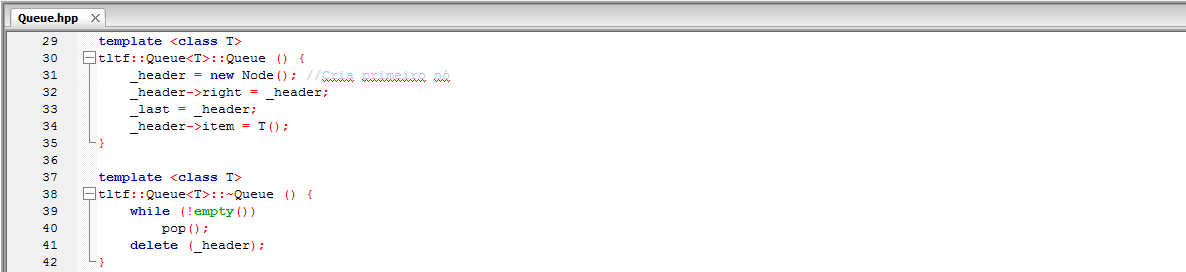
\includegraphics[width=4.7209in,height=2.7083in]{T1-img11.png} \par}

{\centering
\textit{\textcolor[rgb]{0.49803922,0.49803922,0.49803922}{Imagem 3.1 –
Construtor e destrutor}}
\par}

O método construtor cria um novo nó em Header. Como a fila está sendo
inicializada, o nó a direita do Header será ele mesmo. Dessa forma,
sempre que o nó seguinte ao Header for ele mesmo, a fila está vázia.

O método destrutor, pensando na reusabilidade e portabilidade, utiliza a
função pop() para liberar a memória dos elementos da fila. Quando
restar apenas o nó Header, este é deletado como os outros nós.


\bigskip

{\centering 
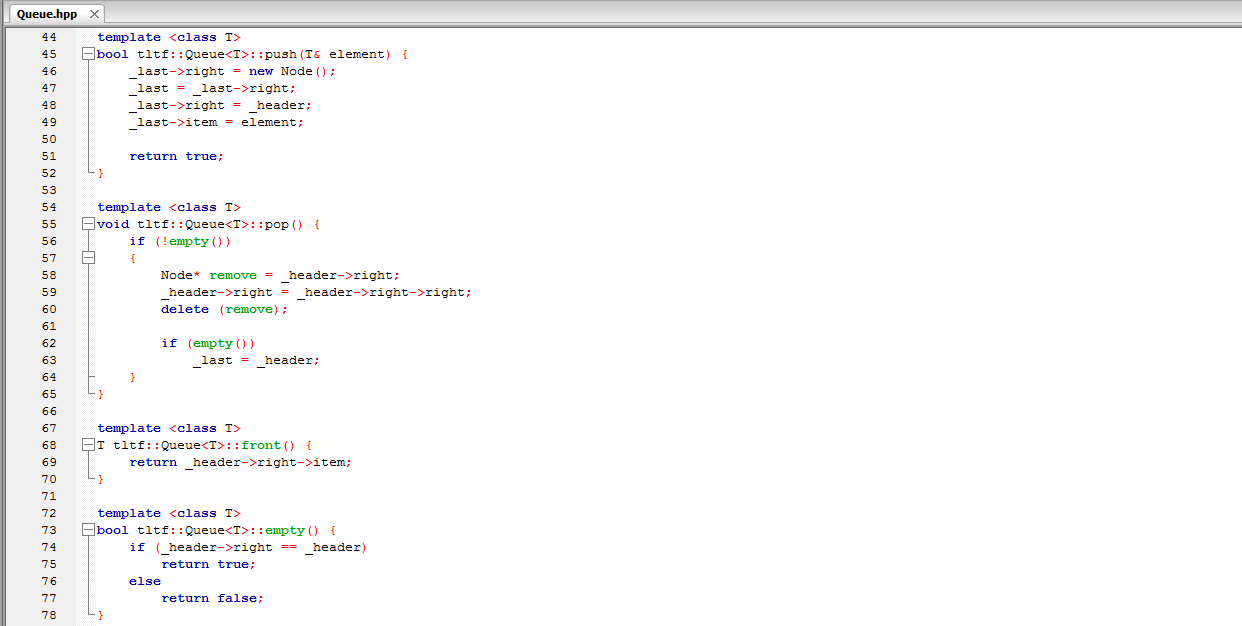
\includegraphics[width=3.3602in,height=4.0193in]{T1-img12.png} \par}

{\centering
\textit{\textcolor[rgb]{0.49803922,0.49803922,0.49803922}{Imagem 3.2 –
Inserção, remoção, primeiro elemento, vazia}}
\par}


\bigskip

Função pop() irá deletar o primeiro elemento da fila. Nesta função, o
header é utilizado tanto para verificar se a fila está vazia, quanto
para encontrar o primeiro nó da fila. Verificado que a fila não está
vazia, atualiza-se o ponteiro\textit{ right} do Header. Agora, o
primeiro elemento é o antigo segundo elemento da fila.

{\centering 
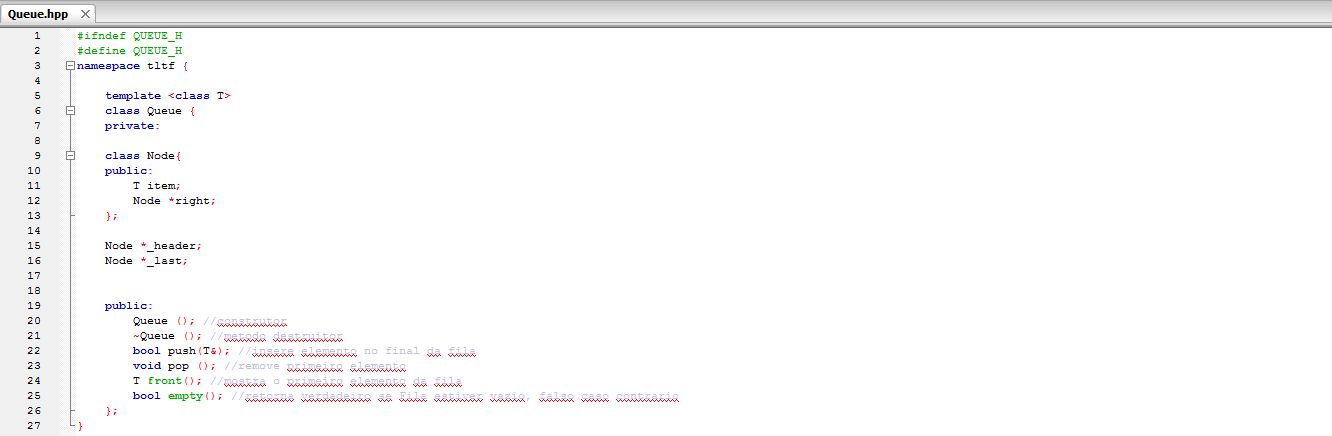
\includegraphics[width=5.9402in,height=3.698in]{T1-img13.png} \par}

{\centering
\textit{\textcolor[rgb]{0.34901962,0.34901962,0.34901962}{Imagem 3.3 –
Declaração da Fila}}
\par}


\bigskip

\textbf{MemoryQueue}

Entretanto, a estrutura Fila não atende aos requisitos do jogo proposto.
A regra do jogo requer que haja alguma forma de manter o último
elemento retirado na memória, para que este possa ser comparado com a
frente da fila. Nesse sentido, implementou-se uma Classe
\textit{MemoryQueue}, responsável por encapsular uma “Fila normal”
(descrita na seção anterior) junto com o último elemento retirado da
fila, uma espécie de “memória”.

É válido notar que a criação desse tipo de estrutura seria inevitável.
Porém, a estrutura que ela encapsula poderia ser do tipo Lista. Isto é,
tanto a Fila quanto a Lista possuem propriedades vantajosas à
implementação desse jogo. A Fila, permite naturalmente o acesso ao
elemento que está “à frente”. A Lista, permite o acesso à dois (ou
mais) elementos. Para a implementação desse jogo, para estar de acordo
tanto com o contexto desse projeto quanto com a opinião de seus
criadores, utilizou-se o encapsulamento de uma Fila.

A imagem 4.1 ilustra melhor o que acontece na MemoryQueue a cada
interação:


\bigskip

{\centering\itshape\color[rgb]{0.26666668,0.32941177,0.41568628}
 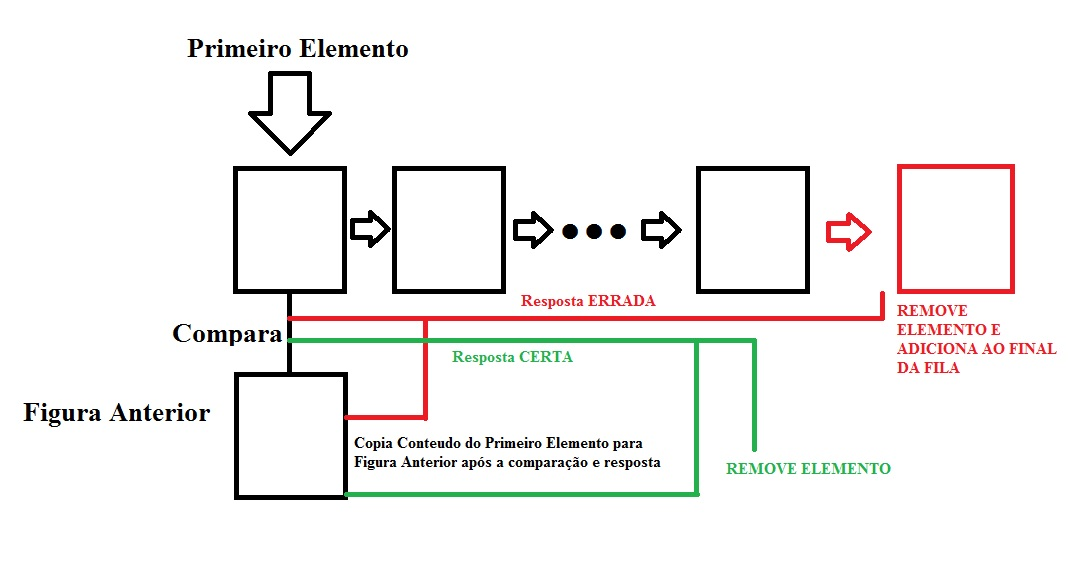
\includegraphics[width=5.8957in,height=3.1165in]{T1-img14.jpg} 
\ Imagem 4. 1 - Demonstração Lúdica de como a Fila é utilizada no jogo
\par}


\bigskip


\bigskip

\textbf{Como a Lista é implementada e utilizada?}

Durante o desenvolvimento do projeto, foi necessário reunir alguns
elementos em uma estrutura do tipo Lista. Inicialmente, utilizou-se a
implementação do container vector, da STL. Porém, os requisitos da
Lista utilizada estavam muito aquém da complexidade por trás de tal
container. Assim, considerando o contexto em que se insere esse
trabalho, optou-se pela realização da implementação de uma Lista que se
enquadrasse exatamente no projeto. 

A estrutura requisitada nada mais era do que um array de tamanho fixo
que tivesse embutida a informação de quantos elementos estão
armazenados. Dessa forma, foi criado justamente uma classe List que
encapsula essas duas informações: elementos, e quantidade de elementos.

Como era suficiente uma estrutura de tamanho fixo, não foi necessário
fazer re-alocamentos de memória. É de destaque a implementação de dois
métodos, cuja necessidade surgiu da proposta de que essa nova estrutura
deveria substituir a solução anterior (std::vector) sem alterar o
código que dependia do acesso a essas informações.

Esses dois métodos foram:

\liststyleWWNumvi
\begin{itemize}
\item O operador de member access []:
\end{itemize}
\foreignlanguage{english}{\textcolor[rgb]{0.3254902,0.5058824,0.20784314}{T\&
}}\foreignlanguage{english}{\textcolor[rgb]{0.3372549,0.6117647,0.8392157}{operator}}\foreignlanguage{english}{\textcolor[rgb]{0.7058824,0.7058824,0.7058824}{[](}}\foreignlanguage{english}{\textcolor[rgb]{0.3254902,0.5058824,0.20784314}{size\_t
pos}}\foreignlanguage{english}{\textcolor[rgb]{0.7058824,0.7058824,0.7058824}{)}}\foreignlanguage{english}{\textcolor[rgb]{0.8627451,0.8627451,0.8627451}{
}}\foreignlanguage{english}{\textcolor[rgb]{0.3372549,0.6117647,0.8392157}{const;}}

\liststyleWWNumvi
\begin{itemize}
\item E um construtor Inicializador de Lista, inserido no C++ 11:
\end{itemize}
\foreignlanguage{english}{\textcolor[rgb]{0.3254902,0.5058824,0.20784314}{List(std::initializer\_list{\textless}T{\textgreater}
args);}}

\foreignlanguage{english}{\ \ \ \  \ \ \ }Assim, é possível inicializar
a Lista da seguinte forma:

\ \ \ \ \ \ \foreignlanguage{english}{\textcolor[rgb]{0.3372549,0.6117647,0.8392157}{const}}\foreignlanguage{english}{\textcolor[rgb]{0.8627451,0.8627451,0.8627451}{
}}\foreignlanguage{english}{\textcolor[rgb]{0.3254902,0.5058824,0.20784314}{tltf::List}}\foreignlanguage{english}{\textcolor[rgb]{0.7058824,0.7058824,0.7058824}{{\textless}}}\foreignlanguage{english}{\textcolor[rgb]{0.3372549,0.6117647,0.8392157}{char}}\foreignlanguage{english}{\textcolor[rgb]{0.7058824,0.7058824,0.7058824}{*{\textgreater}}}\foreignlanguage{english}{\textcolor[rgb]{0.8627451,0.8627451,0.8627451}{
}}\foreignlanguage{english}{\textcolor[rgb]{0.3254902,0.5058824,0.20784314}{tltf::Config::imagesPaths
}}\foreignlanguage{english}{\textcolor[rgb]{0.7058824,0.7058824,0.7058824}{=}}\foreignlanguage{english}{\textcolor[rgb]{0.8627451,0.8627451,0.8627451}{
}}\foreignlanguage{english}{\textcolor[rgb]{0.7058824,0.7058824,0.7058824}{\{}}

\foreignlanguage{english}{\textcolor[rgb]{0.8627451,0.8627451,0.8627451}{\ \ \ \ \ \ \ \ }}\foreignlanguage{english}{\textcolor[rgb]{0.8392157,0.6156863,0.52156866}{{\textquotedbl}images/image0.png{\textquotedbl}}}\foreignlanguage{english}{\textcolor[rgb]{0.7058824,0.7058824,0.7058824}{,}}

\foreignlanguage{english}{\textcolor[rgb]{0.8627451,0.8627451,0.8627451}{\ \ \ \ \ \ \ \ }}\foreignlanguage{english}{\textcolor[rgb]{0.8392157,0.6156863,0.52156866}{{\textquotedbl}images/image1.png{\textquotedbl}}}\foreignlanguage{english}{\textcolor[rgb]{0.7058824,0.7058824,0.7058824}{,}}

\foreignlanguage{english}{\textcolor[rgb]{0.8627451,0.8627451,0.8627451}{\ \ \ \ \ \ \ \ }}\foreignlanguage{english}{\textcolor[rgb]{0.8392157,0.6156863,0.52156866}{{\textquotedbl}images/image2.png{\textquotedbl}}}\foreignlanguage{english}{\textcolor[rgb]{0.7058824,0.7058824,0.7058824}{,}}

\foreignlanguage{english}{\textcolor[rgb]{0.8627451,0.8627451,0.8627451}{\ \ \ \ \ \ \ \ }}\foreignlanguage{english}{\textcolor[rgb]{0.8392157,0.6156863,0.52156866}{{\textquotedbl}images/image3.png{\textquotedbl}}}

\textcolor[rgb]{0.7058824,0.7058824,0.7058824}{\};}

\textbf{Como o Mapa é utilizado?}

Um Mapa é uma estrutura de dados que permite o armazenamento de
elementos “indexados” por uma chave, normalmente única. Externamente, e
para fins didáticos, se parece com um vetor que, ao invés de ter
índices numéricos e acessar o elemento “na posição I”, permite ter
qualquer tipo de objeto como índice e acessa o elemento “com a chave
K”.

Internamente, entretanto, os mapas possuem comportamentos diferentes.
Eles costumam ordenar seus dados em relação à chave e, para manter
eficiência nas operações de inserção, consulta e remoção, são
implementados com árvores binárias balanceadas.

Na implementação desse jogo, foi utilizado o std::map, um container da
STL. Dessa forma, pode-se definir identificadores às imagens utilizadas
e manipuladas pelo jogo. São utilizados dois maps. Um relaciona o
identificador da imagem ao endereço (relative-path) de seu arquivo no
sistema. O outro, relaciona um identificador (o mesmo, por comodidade e
coerência) à um objeto da Classe Image.

Dessa forma, reúne-se todas as imagens do sistema em uma única estrutura
de dados, que assegura velocidade na manipulação desses objetos. Ex:

\textcolor[rgb]{0.8392157,0.6156863,0.52156866}{systemImages[}\textcolor[rgb]{0.3372549,0.6117647,0.8392157}{”name”}\textcolor[rgb]{0.8392157,0.6156863,0.52156866}{].}\textcolor[rgb]{0.3254902,0.5058824,0.20784314}{getBitmap}\textcolor[rgb]{0.8392157,0.6156863,0.52156866}{();}


\bigskip


\bigskip


\bigskip

\textbf{Observações e Comentários:}

Essa seção reúne pequenas informações quanto ao processo de
desenvolvimento do jogo.

\liststyleWWNumvi
\begin{itemize}
\item O Jogo em sua versão atual é dependente da dll
allegro-5.0.10-monolith-mt.dll. Vários esforços foram realizados
buscando eliminar essa necessidade. A ideia central é fazer um
static-linkage com as bilibotecas *-static-mt.dll disponibilizadas pelo
Allegro. Entretanto, não foi encontrado nenhum caso de sucesso. Outra
alternativa seria utilizar programas injetores de dlls em executáveis.
Testou-se esse procedimento com o programa PE-Inject, mas sem sucesso.
Exemplo de insucesso no static-linkage:
\url{https://www.allegro.cc/forums/thread/613981};
\item Para atribuir um ícone ao executável, seguiu-se o procedimento
descrito em \url{https://www.allegro.cc/forums/thread/601721Monolith};
\item Foi utilizado o addon PhysicsFS do Allegro, uma camada de
abstração do PhysicsFS, que por sua vez, permite acesso à vários tipos
de arquivos. Dessa forma, pode-se ler arquivos zipados pelos mesmos
métodos de acesso de arquivos do Allegro. Veja:
\url{https://www.allegro.cc/manual/5/physfs.html};
\item Utilizou-se a função setResourceArchive() no arquivo
TheLastTooFast.cpp. Tal função está descrita em
\url{https://www.allegro.cc/forums/thread/614268}, e faz com que o
working-directory da aplicação seja mudado para a pasta em que se
encontra o executável. Assim, pode-se utilizar relative-paths para
referenciar os arquivos usados pelo jogo;
\item Foi proposta a implementação de uma “memória” de scores. Porém,
restringiu-se posteriormente o escopo da aplicação, eliminando essa
funcionalidade. Mesmo assim, parte do código que seria utilizado
encontra-se comentado no código-fonte, sob a diretriz TODO;
\item Toda a lógica da Interface Gráfica está embutida em um único
arquivo (TheLastTooFast.cpp), incluindo as funções referentes à cada
tela do jogo. Essa implementação não permite grande escalabilidade
referente, principalmente, ao número de telas. Uma possível
alternativa, seria criar uma Classe que encapsulasse, no mínimo, os
métodos draw() e checkEvents(). Entretanto, não houve tal necessidade
de refatoração do sistema devido sua relativa baixa complexidade.
\end{itemize}

\bigskip


\bigskip


\bigskip


\bigskip


\bigskip


\bigskip


\bigskip


\bigskip


\bigskip


\bigskip


\bigskip


\bigskip


\bigskip

\textbf{Conclusão:}

O desenvolvimento do projeto contribuiu largamente para a fixação e
compreensão do conteúdo apresentado na disciplina Estruturas de Dados.
Além disso, possibilitou o uso de conhecimentos adquiridos
paralelamente em outras disciplinas, como o uso (mesmo que de forma
informal) de diagramas que são apresentados na disciplina de Introdução
aos Sistemas de Informação.

As dificuldades maiores se deram quanto a utilização do Allegro para o
desenvolvimento gráfico. A falta de uma Engine com editor gráfico faz
com que cada imagem tenha ter sua posição calculada com precisão, isso
é claro, com o objetivo de manter uma estética de jogo agradável ao
usuário. Além disso, o Allegro não era conhecido por ninguém do grupo.

Apesar das dificuldades, essencialmente no desenvolvimento da interface
gráfica, o desenvolvimento do jogo foi extremamente prazeroso e
gratificante a cada pequeno passo conquistado. O auge se deu ao ver o
jogo funcionando e mais, ao ver pessoas se divertindo com ele. 
\end{document}
